\documentclass[a4paper, 11pt]{article}

% Nécessaire
\usepackage[utf8]{inputenc}
\usepackage[T1]{fontenc}
\usepackage{lmodern}

% Biblio
\usepackage{natbib}
\bibliographystyle{abbrvnat}
\usepackage{hypernat}
\bibpunct{\textcolor{blue}{[}}{\textcolor{blue}{]}}{}{a}{\textcolor{blue}{,}}{;}

\usepackage[french]{babel}
\usepackage{amsmath, amsthm}
\usepackage{amsfonts,amssymb}

% Marge
\usepackage{geometry}
\geometry{margin={2.2cm ,2cm}}

% Figures, graphiques
\usepackage{graphicx}
\usepackage{epsfig}
\usepackage{caption}

% Surlignage
\usepackage{alltt}

\usepackage{xcolor}
\usepackage{soul}
\usepackage{color}
\usepackage{colortbl}

% Indicatrice
\usepackage{dsfont}

\usepackage{multirow}
\usepackage{eurosym}
\usepackage{extarrows}
\usepackage[colorlinks=true, citecolor=blue, linkcolor=.]{hyperref}

% Graphique
\usepackage{tikz}


% Titre
\title{Calibration du modèle en utlisant des inflorescences aux stades C/D/E}
\author{}
\date{}



\begin{document}
 \maketitle
 
 \section{Les inflorescences}
 
 Pour simuler les dynamiques d'inflorescences aux stades C/D/E, il faut partir des dates de débourrements.
 Deux choix sont possibles, soit utiliser les débourrements observés et mis à l'échelle, soit utiliser les débourrements simulés.
 (Pour l'enherbement haut, les débourrements simulés seront utilisés.)
 Pour les modalités ER et PS, les différences sont visibles sur la figure~\ref{fig:erps}.
 \begin{figure}[ht]
  \centering
  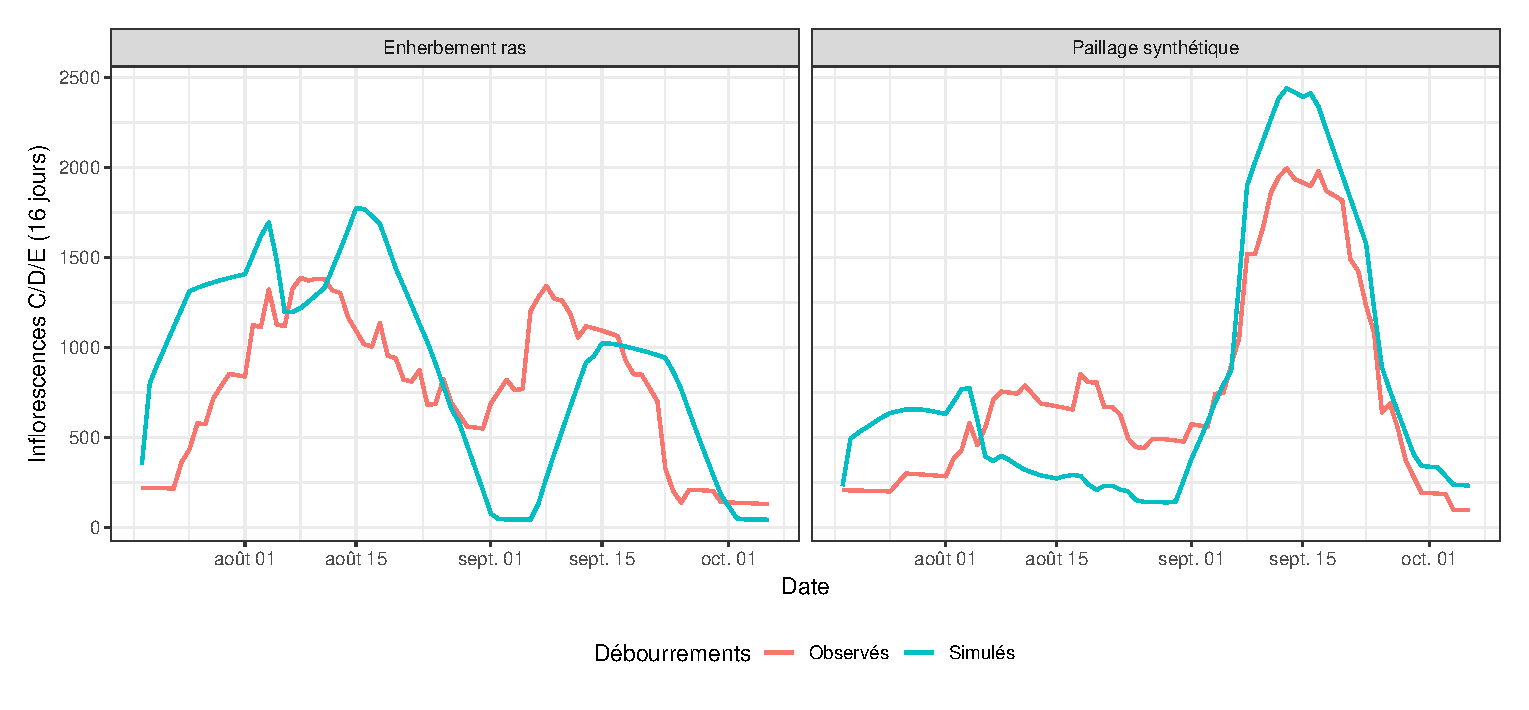
\epsfig{file = plots/inflosCDEerps.eps, scale = 0.65}
  \caption{Comparaison des dynamiques d'inflorescences C/D/E pour les sols ER et PS.}
  \label{fig:erps}
 \end{figure}
 
 On constate des différences entre les dynamiques d'inflorescences en fonction des débourrements observés et simulés.
 On choisira celles issues des débourrements observés pour rester au plus près de la réalité.
 
 \section{Les résultats}
 
 Les résultats produits par la figure~\ref{fig:arg1} sont produit par les paramètres :
 
 \begin{center}
\begin{tabular}{lllllll}
$\gamma$ & $p_m$ & $\mu_{\text{ER}}$ & $\mu_{\text{EH}}$ & $k$ & \texttt{stock} & \texttt{reproduction}\\
0.072 & 0.722 & 0.028 & 0.060 & 14.254 & 19462 & 9.805
 \end{tabular}
 \end{center}

 
  \begin{figure}[ht]
  \centering
  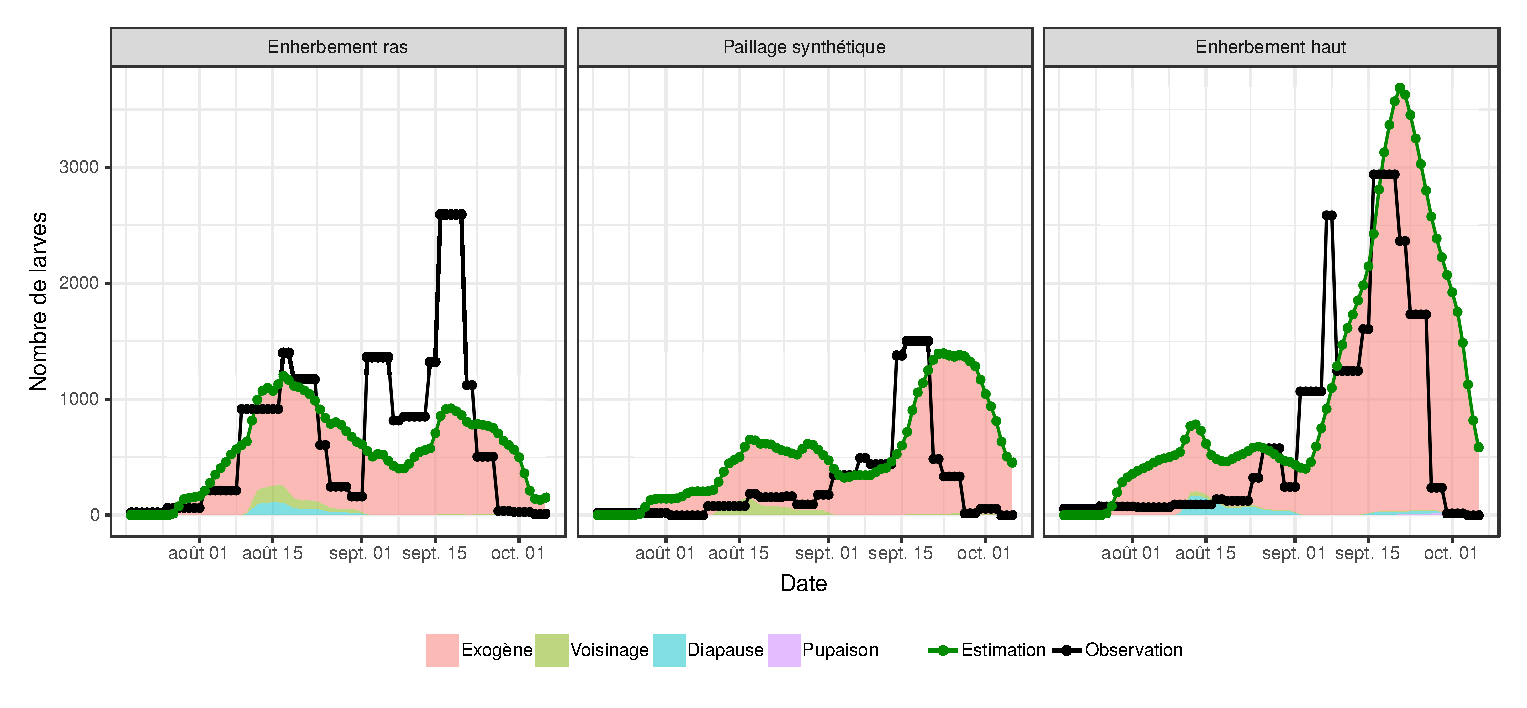
\epsfig{file = plots/CDEarg1.eps, scale = 0.65}
  \caption{}
  \label{fig:arg1}
 \end{figure}
 
 Les résultats produits par la figure~\ref{fig:arg2} sont produit par les paramètres :
 
  \begin{center}
\begin{tabular}{lllllll}
$\gamma$ & $p_m$ & $\mu_{\text{ER}}$ & $\mu_{\text{EH}}$ & $k$ & \texttt{stock} & \texttt{reproduction}\\
0.049 & 0.908 & 0.841 & 0.004 & 5.427 & 11018 & 5.472
 \end{tabular}
 \end{center}
 
 
  \begin{figure}[ht]
  \centering
  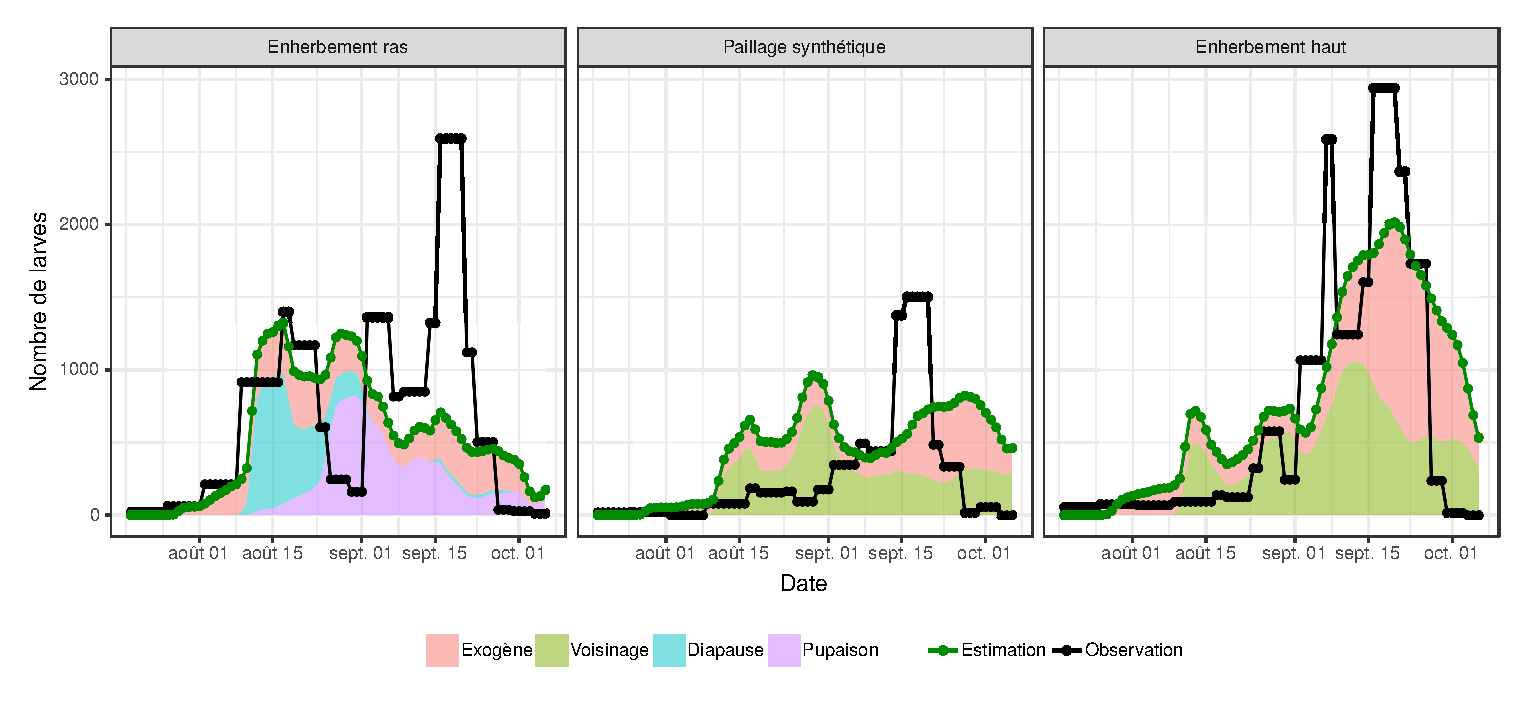
\epsfig{file = plots/CDEarg2.eps, scale = 0.65}
  \caption{}
  \label{fig:arg2}
 \end{figure}
 
\end{document}

